\documentclass{extbook}[14pt]
\usepackage{multicol, enumerate, enumitem, hyperref, color, soul, setspace, parskip, fancyhdr, amssymb, amsthm, amsmath, latexsym, units, mathtools}
\everymath{\displaystyle}
\usepackage[headsep=0.5cm,headheight=0cm, left=1 in,right= 1 in,top= 1 in,bottom= 1 in]{geometry}
\usepackage{dashrule}  % Package to use the command below to create lines between items
\newcommand{\litem}[1]{\item #1

\rule{\textwidth}{0.4pt}}
\pagestyle{fancy}
\lhead{}
\chead{Answer Key for Makeup Progress Quiz 2 Version ALL}
\rhead{}
\lfoot{2790-1423}
\cfoot{}
\rfoot{Summer C 2021}
\begin{document}
\textbf{This key should allow you to understand why you choose the option you did (beyond just getting a question right or wrong). \href{https://xronos.clas.ufl.edu/mac1105spring2020/courseDescriptionAndMisc/Exams/LearningFromResults}{More instructions on how to use this key can be found here}.}

\textbf{If you have a suggestion to make the keys better, \href{https://forms.gle/CZkbZmPbC9XALEE88}{please fill out the short survey here}.}

\textit{Note: This key is auto-generated and may contain issues and/or errors. The keys are reviewed after each exam to ensure grading is done accurately. If there are issues (like duplicate options), they are noted in the offline gradebook. The keys are a work-in-progress to give students as many resources to improve as possible.}

\rule{\textwidth}{0.4pt}

\begin{enumerate}\litem{
Determine the horizontal and/or oblique asymptotes in the rational function below.
\[ f(x) = \frac{10x^{3} -59 x^{2} +61 x + 60}{-10x^{3} +3 x^{2} -27 x -36} \]The solution is \( \text{Horizontal Asymptote of } y = -1.000  \), which is option D.\begin{enumerate}[label=\Alph*.]
\item \( \text{Horizontal Asymptote of } y = 0  \)

This corresponds to using the rule for Horizontal Asymptote when the degree of the denominator is larger than the numerator.
\item \( \text{Vertical Asymptote of } y = 1.500  \)

This corresponds to the hole at $x = 1.500$.
\item \( \text{None of the above} \)

This corresponds to believing there should be an oblique asymptote.
\item \( \text{Horizontal Asymptote of } y = -1.000  \)

* This is the correct option.
\item \( \text{Vertical Asymptote of } y = 4  \)

This corresponds to the hole at $x = 4$.
\end{enumerate}

\textbf{General Comment:} We have a Horizontal Asymptote if the degree of the numerator is smaller than or equal to the degree of the denominator. We have an Oblique Asymptote if the degree of the numerator is larger than the degree of the denominator. We cannot have both!
}
\litem{
Determine the vertical asymptotes and holes in the rational function below.
\[ f(x) = \frac{8x^{3} -50 x^{2} +93 x -45}{8x^{2} -10 x -25} \]The solution is \( \text{Vertical Asymptote of } x = -1.25 \text{ and hole at } x = 2.5 \), which is option B.\begin{enumerate}[label=\Alph*.]
\item \( \text{Vertical Asymptote of } x = 1.0 \text{ and hole at } x = 2.5 \)

This corresponds to mixing vertical and horizontal asymptotes.
\item \( \text{Vertical Asymptote of } x = -1.25 \text{ and hole at } x = 2.5 \)

This is the correct answer.
\item \( \text{Holes at } x = -1.25 \text{ and } x = 2.5 \text{ with no vertical asymptotes.} \)

This corresponds to considering where the denominator is equal to 0 as holes.
\item \( \text{Vertical Asymptotes of } x = -1.25 \text{ and } x = 2.5 \text{ with no holes.} \)

This corresponds to not factoring out the hole.
\item \( \text{Vertical Asymptotes of } x = -1.25 \text{ and } x = 0.75 \text{ with a hole at } x = 2.5 \)

This corresponds to setting the numerator equal to 0.
\end{enumerate}

\textbf{General Comment:} Remember to factor the numerator and denominator. Any factors that cancel are holes in the function. The zeros left in the denominator are the vertical asymptotes.
}
\litem{
Which of the following functions \textit{could} be the graph below?

\begin{center}
    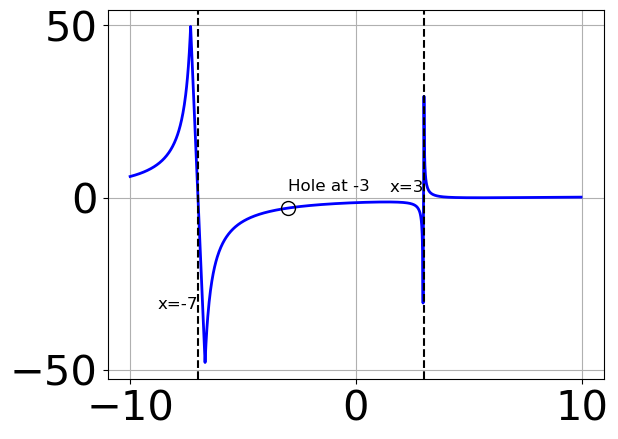
\includegraphics[width=0.5\textwidth]{../Figures/identifyGraphOfRationalFunctionCopyA.png}
\end{center}


The solution is \( f(x)=\frac{x^{3} -8.0 x^{2} -3.0 x + 90.0}{x^{3} +7.0 x^{2} -9.0 x -63.0} \), which is option B.\begin{enumerate}[label=\Alph*.]
\item \( f(x)=\frac{x^{3} +8.0 x^{2} -3.0 x -90.0}{x^{3} -7.0 x^{2} -9.0 x + 63.0} \)

Remember that factors are written as $x-z$. For example, the zero $x=-7$ corresponds to the factor $x-(-7)$.
\item \( f(x)=\frac{x^{3} -8.0 x^{2} -3.0 x + 90.0}{x^{3} +7.0 x^{2} -9.0 x -63.0} \)

This is the correct answer!
\item \( f(x)=\frac{x^{3} +13.0 x^{2} +52.0 x + 60.0}{x^{3} -7.0 x^{2} -9.0 x + 63.0} \)

You treated all of the zeros in the denominator as vertical asmptotes when some of them were holes and wrote factors as $x+z$.
\item \( f(x)=\frac{x^{3} -10.0 x^{2} +19.0 x + 30.0}{x^{3} +7.0 x^{2} -9.0 x -63.0} \)

You treated all of the zeros in the denominator as vertical asymptotes when some of them were holes!
\item \( \text{None of the above are possible equations for the graph.} \)

If you believe none of the functions above could be the graph, please contact the coordinator.
\end{enumerate}

\textbf{General Comment:} We want to factor the numerator and denominator to determine which zeros in the denominator are vertical asympototes and which are holes.
}
\litem{
Determine the horizontal and/or oblique asymptotes in the rational function below.
\[ f(x) = \frac{12x^{3} -65 x^{2} +74 x -24}{3x^{2} -11 x + 6} \]The solution is \( y = 4x -7 \), which is option A.\begin{enumerate}[label=\Alph*.]
\item \( \text{Oblique Asymptote of } y = 4x -7. \)

This is the correct answer.
\item \( \text{Horizontal Asymptote of } y = 4.0 \text{ and Oblique Asymptote of } y = 4x -7 \)

This corresponds to believing there can be both a horizontal and oblique asymptote.
\item \( \text{Horizontal Asymptote of } y = 3.0 \text{ and Oblique Asymptote of } y = 4x -7 \)

This corresponds to believing there can be both a horizontal and oblique asymptote AND mixing up horizontal/vertical asymoptote.
\item \( \text{Horizontal Asymptote of } y = 4.0  \)

This corresponds to using rule for Horizontal Asymptote when degree of numerator and denominator match.
\item \( \text{Horizontal Asymptote at } y = 3.0 \)

This corresponds to considering where the denominator is equal to 0 as horizontal asymptote.
\end{enumerate}

\textbf{General Comment:} We have a Horizontal Asymptote if the degree of the numerator is smaller than or equal to the degree of the denominator. We have an Oblique Asymptote if the degree of the numerator is larger than the degree of the denominator. We cannot have both!
}
\litem{
Which of the following functions \textit{could} be the graph below?

\begin{center}
    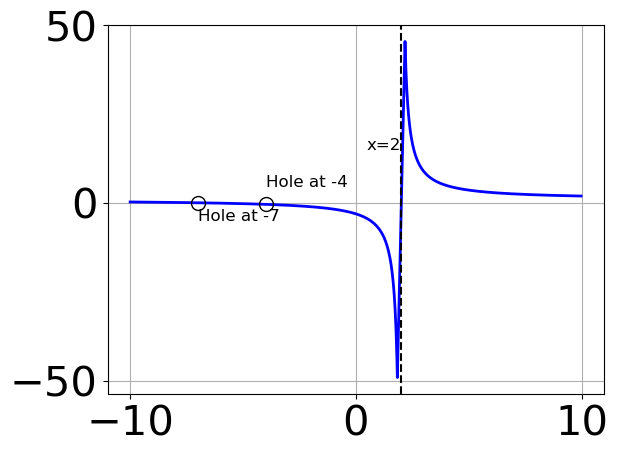
\includegraphics[width=0.5\textwidth]{../Figures/identifyGraphOfRationalFunctionA.png}
\end{center}


The solution is \( f(x)=\frac{x^{3} +17.0 x^{2} +94.0 x + 168.0}{x^{3} +9.0 x^{2} +6.0 x -56.0} \), which is option B.\begin{enumerate}[label=\Alph*.]
\item \( f(x)=\frac{x^{3} +14.0 x^{2} +63.0 x + 90.0}{x^{3} +9.0 x^{2} +6.0 x -56.0} \)

You treated all of the zeros in the denominator as vertical asymptotes when some of them were holes!
\item \( f(x)=\frac{x^{3} +17.0 x^{2} +94.0 x + 168.0}{x^{3} +9.0 x^{2} +6.0 x -56.0} \)

This is the correct answer!
\item \( f(x)=\frac{x^{3} -17.0 x^{2} +94.0 x -168.0}{x^{3} -9.0 x^{2} +6.0 x + 56.0} \)

Remember that factors are written as $x-z$. For example, the zero $x=2$ corresponds to the factor $x-(2)$.
\item \( f(x)=\frac{x^{3} -7.0 x^{2} -24.0 x + 180.0}{x^{3} -9.0 x^{2} +6.0 x + 56.0} \)

You treated all of the zeros in the denominator as vertical asmptotes when some of them were holes and wrote factors as $x+z$.
\item \( \text{None of the above are possible equations for the graph.} \)

If you believe none of the functions above could be the graph, please contact the coordinator.
\end{enumerate}

\textbf{General Comment:} We want to factor the numerator and denominator to determine which zeros in the denominator are vertical asympototes and which are holes.
}
\litem{
Determine the vertical asymptotes and holes in the rational function below.
\[ f(x) = \frac{8x^{3} -18 x^{2} -11 x + 30}{16x^{2} +32 x + 15} \]The solution is \( \text{Vertical Asymptote of } x = -0.75 \text{ and hole at } x = -1.25 \), which is option B.\begin{enumerate}[label=\Alph*.]
\item \( \text{Vertical Asymptotes of } x = -0.75 \text{ and } x = 1.5 \text{ with a hole at } x = -1.25 \)

This corresponds to setting the numerator equal to 0.
\item \( \text{Vertical Asymptote of } x = -0.75 \text{ and hole at } x = -1.25 \)

This is the correct answer.
\item \( \text{Vertical Asymptote of } x = 0.5 \text{ and hole at } x = -1.25 \)

This corresponds to mixing vertical and horizontal asymptotes.
\item \( \text{Vertical Asymptotes of } x = -0.75 \text{ and } x = -1.25 \text{ with no holes.} \)

This corresponds to not factoring out the hole.
\item \( \text{Holes at } x = -0.75 \text{ and } x = -1.25 \text{ with no vertical asymptotes.} \)

This corresponds to considering where the denominator is equal to 0 as holes.
\end{enumerate}

\textbf{General Comment:} Remember to factor the numerator and denominator. Any factors that cancel are holes in the function. The zeros left in the denominator are the vertical asymptotes.
}
\litem{
Determine the horizontal and/or oblique asymptotes in the rational function below.
\[ f(x) = \frac{9x^{3} -18 x^{2} -64 x -32}{3x^{2} +19 x + 20} \]The solution is \( y = 3x -25 \), which is option E.\begin{enumerate}[label=\Alph*.]
\item \( \text{Horizontal Asymptote of } y = -5.0 \text{ and Oblique Asymptote of } y = 3x -25 \)

This corresponds to believing there can be both a horizontal and oblique asymptote AND mixing up horizontal/vertical asymoptote.
\item \( \text{Horizontal Asymptote of } y = 3.0 \text{ and Oblique Asymptote of } y = 3x -25 \)

This corresponds to believing there can be both a horizontal and oblique asymptote.
\item \( \text{Horizontal Asymptote at } y = -5.0 \)

This corresponds to considering where the denominator is equal to 0 as horizontal asymptote.
\item \( \text{Horizontal Asymptote of } y = 3.0  \)

This corresponds to using rule for Horizontal Asymptote when degree of numerator and denominator match.
\item \( \text{Oblique Asymptote of } y = 3x -25. \)

This is the correct answer.
\end{enumerate}

\textbf{General Comment:} We have a Horizontal Asymptote if the degree of the numerator is smaller than or equal to the degree of the denominator. We have an Oblique Asymptote if the degree of the numerator is larger than the degree of the denominator. We cannot have both!
}
\litem{
Determine the horizontal and/or oblique asymptotes in the rational function below.
\[ f(x) = \frac{15x^{3} +26 x^{2} -51 x + 18}{-15x^{3} +8 x^{2} +3 x + 18} \]The solution is \( \text{Horizontal Asymptote of } y = -1.000  \), which is option E.\begin{enumerate}[label=\Alph*.]
\item \( \text{Vertical Asymptote of } y = -0.667  \)

This corresponds to the hole at $x = -0.667$.
\item \( \text{None of the above} \)

This corresponds to believing there should be an oblique asymptote.
\item \( \text{Horizontal Asymptote of } y = 0  \)

This corresponds to using the rule for Horizontal Asymptote when the degree of the denominator is larger than the numerator.
\item \( \text{Vertical Asymptote of } y = -3  \)

This corresponds to the hole at $x = -3$.
\item \( \text{Horizontal Asymptote of } y = -1.000  \)

* This is the correct option.
\end{enumerate}

\textbf{General Comment:} We have a Horizontal Asymptote if the degree of the numerator is smaller than or equal to the degree of the denominator. We have an Oblique Asymptote if the degree of the numerator is larger than the degree of the denominator. We cannot have both!
}
\litem{
Determine the vertical asymptotes and holes in the rational function below.
\[ f(x) = \frac{9x^{3} -24 x^{2} +4 x + 16}{12x^{2} +23 x + 10} \]The solution is \( \text{Vertical Asymptote of } x = -1.25 \text{ and hole at } x = -0.667 \), which is option E.\begin{enumerate}[label=\Alph*.]
\item \( \text{Holes at } x = -1.25 \text{ and } x = -0.667 \text{ with no vertical asymptotes.} \)

This corresponds to considering where the denominator is equal to 0 as holes.
\item \( \text{Vertical Asymptotes of } x = -1.25 \text{ and } x = -0.667 \text{ with no holes.} \)

This corresponds to not factoring out the hole.
\item \( \text{Vertical Asymptotes of } x = -1.25 \text{ and } x = 1.333 \text{ with a hole at } x = -0.667 \)

This corresponds to setting the numerator equal to 0.
\item \( \text{Vertical Asymptote of } x = 0.75 \text{ and hole at } x = -0.667 \)

This corresponds to mixing vertical and horizontal asymptotes.
\item \( \text{Vertical Asymptote of } x = -1.25 \text{ and hole at } x = -0.667 \)

This is the correct answer.
\end{enumerate}

\textbf{General Comment:} Remember to factor the numerator and denominator. Any factors that cancel are holes in the function. The zeros left in the denominator are the vertical asymptotes.
}
\litem{
Determine the vertical asymptotes and holes in the rational function below.
\[ f(x) = \frac{9x^{3} -18 x^{2} -7 x + 20}{6x^{2} +7 x -20} \]The solution is \( \text{Vertical Asymptote of } x = -2.5 \text{ and hole at } x = 1.333 \), which is option D.\begin{enumerate}[label=\Alph*.]
\item \( \text{Vertical Asymptotes of } x = -2.5 \text{ and } x = 1.667 \text{ with a hole at } x = 1.333 \)

This corresponds to setting the numerator equal to 0.
\item \( \text{Vertical Asymptote of } x = 1.5 \text{ and hole at } x = 1.333 \)

This corresponds to mixing vertical and horizontal asymptotes.
\item \( \text{Vertical Asymptotes of } x = -2.5 \text{ and } x = 1.333 \text{ with no holes.} \)

This corresponds to not factoring out the hole.
\item \( \text{Vertical Asymptote of } x = -2.5 \text{ and hole at } x = 1.333 \)

This is the correct answer.
\item \( \text{Holes at } x = -2.5 \text{ and } x = 1.333 \text{ with no vertical asymptotes.} \)

This corresponds to considering where the denominator is equal to 0 as holes.
\end{enumerate}

\textbf{General Comment:} Remember to factor the numerator and denominator. Any factors that cancel are holes in the function. The zeros left in the denominator are the vertical asymptotes.
}
\litem{
Determine the horizontal and/or oblique asymptotes in the rational function below.
\[ f(x) = \frac{9x^{3} +36 x^{2} +44 x + 16}{3x^{3} +20 x^{2} +48 x + 32} \]The solution is \( \text{Horizontal Asymptote of } y = 3.000  \), which is option A.\begin{enumerate}[label=\Alph*.]
\item \( \text{Horizontal Asymptote of } y = 3.000  \)

* This is the correct option.
\item \( \text{Horizontal Asymptote of } y = 0  \)

This corresponds to using the rule for Horizontal Asymptote when the degree of the denominator is larger than the numerator.
\item \( \text{Vertical Asymptote of } y = -2  \)

This corresponds to the hole at $x = -2$.
\item \( \text{None of the above} \)

This corresponds to believing there should be an oblique asymptote.
\item \( \text{Vertical Asymptote of } y = -4.000  \)

This corresponds to the hole at $x = -4.000$.
\end{enumerate}

\textbf{General Comment:} We have a Horizontal Asymptote if the degree of the numerator is smaller than or equal to the degree of the denominator. We have an Oblique Asymptote if the degree of the numerator is larger than the degree of the denominator. We cannot have both!
}
\litem{
Determine the vertical asymptotes and holes in the rational function below.
\[ f(x) = \frac{16x^{3} -16 x^{2} -25 x + 25}{12x^{2} +x -20} \]The solution is \( \text{Vertical Asymptote of } x = -1.333 \text{ and hole at } x = 1.25 \), which is option B.\begin{enumerate}[label=\Alph*.]
\item \( \text{Holes at } x = -1.333 \text{ and } x = 1.25 \text{ with no vertical asymptotes.} \)

This corresponds to considering where the denominator is equal to 0 as holes.
\item \( \text{Vertical Asymptote of } x = -1.333 \text{ and hole at } x = 1.25 \)

This is the correct answer.
\item \( \text{Vertical Asymptote of } x = 1.333 \text{ and hole at } x = 1.25 \)

This corresponds to mixing vertical and horizontal asymptotes.
\item \( \text{Vertical Asymptotes of } x = -1.333 \text{ and } x = -1.25 \text{ with a hole at } x = 1.25 \)

This corresponds to setting the numerator equal to 0.
\item \( \text{Vertical Asymptotes of } x = -1.333 \text{ and } x = 1.25 \text{ with no holes.} \)

This corresponds to not factoring out the hole.
\end{enumerate}

\textbf{General Comment:} Remember to factor the numerator and denominator. Any factors that cancel are holes in the function. The zeros left in the denominator are the vertical asymptotes.
}
\litem{
Which of the following functions \textit{could} be the graph below?

\begin{center}
    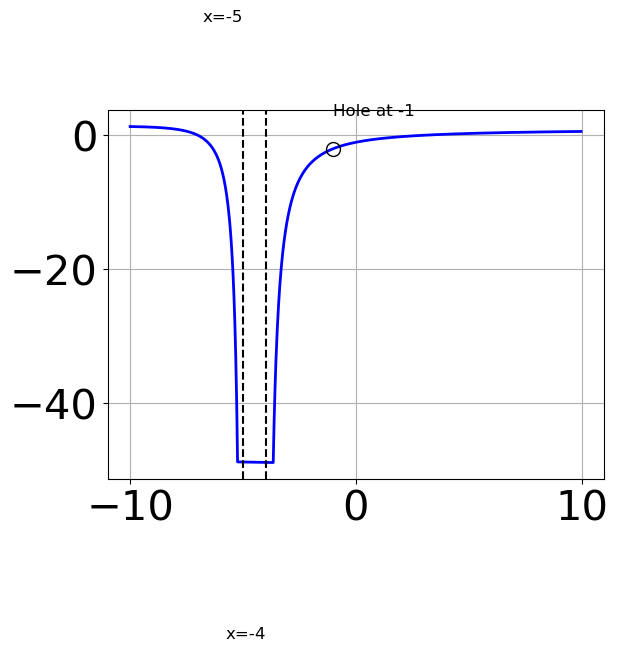
\includegraphics[width=0.5\textwidth]{../Figures/identifyGraphOfRationalFunctionCopyB.png}
\end{center}


The solution is \( f(x)=\frac{x^{3} +5.0 x^{2} -17.0 x -21.0}{x^{3} +10.0 x^{2} +29.0 x + 20.0} \), which is option A.\begin{enumerate}[label=\Alph*.]
\item \( f(x)=\frac{x^{3} +5.0 x^{2} -17.0 x -21.0}{x^{3} +10.0 x^{2} +29.0 x + 20.0} \)

This is the correct answer!
\item \( f(x)=\frac{x^{3} -5.0 x^{2} -17.0 x + 21.0}{x^{3} -10.0 x^{2} +29.0 x -20.0} \)

Remember that factors are written as $x-z$. For example, the zero $x=-5$ corresponds to the factor $x-(-5)$.
\item \( f(x)=\frac{x^{3} -3.0 x^{2} -25.0 x -21.0}{x^{3} -10.0 x^{2} +29.0 x -20.0} \)

You treated all of the zeros in the denominator as vertical asmptotes when some of them were holes and wrote factors as $x+z$.
\item \( f(x)=\frac{x^{3} +3.0 x^{2} -25.0 x + 21.0}{x^{3} +10.0 x^{2} +29.0 x + 20.0} \)

You treated all of the zeros in the denominator as vertical asymptotes when some of them were holes!
\item \( \text{None of the above are possible equations for the graph.} \)

If you believe none of the functions above could be the graph, please contact the coordinator.
\end{enumerate}

\textbf{General Comment:} We want to factor the numerator and denominator to determine which zeros in the denominator are vertical asympototes and which are holes.
}
\litem{
Determine the horizontal and/or oblique asymptotes in the rational function below.
\[ f(x) = \frac{4x^{3} +12 x^{2} -25 x -75}{2x^{2} +13 x + 20} \]The solution is \( y = 2x -7 \), which is option E.\begin{enumerate}[label=\Alph*.]
\item \( \text{Horizontal Asymptote of } y = 2.0  \)

This corresponds to using rule for Horizontal Asymptote when degree of numerator and denominator match.
\item \( \text{Horizontal Asymptote at } y = -4.0 \)

This corresponds to considering where the denominator is equal to 0 as horizontal asymptote.
\item \( \text{Horizontal Asymptote of } y = -4.0 \text{ and Oblique Asymptote of } y = 2x -7 \)

This corresponds to believing there can be both a horizontal and oblique asymptote AND mixing up horizontal/vertical asymoptote.
\item \( \text{Horizontal Asymptote of } y = 2.0 \text{ and Oblique Asymptote of } y = 2x -7 \)

This corresponds to believing there can be both a horizontal and oblique asymptote.
\item \( \text{Oblique Asymptote of } y = 2x -7. \)

This is the correct answer.
\end{enumerate}

\textbf{General Comment:} We have a Horizontal Asymptote if the degree of the numerator is smaller than or equal to the degree of the denominator. We have an Oblique Asymptote if the degree of the numerator is larger than the degree of the denominator. We cannot have both!
}
\litem{
Which of the following functions \textit{could} be the graph below?

\begin{center}
    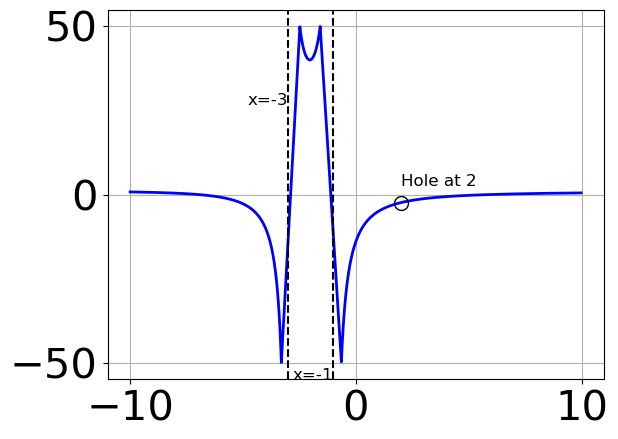
\includegraphics[width=0.5\textwidth]{../Figures/identifyGraphOfRationalFunctionB.png}
\end{center}


The solution is \( f(x)=\frac{x^{3} -1.0 x^{2} -44.0 x + 84.0}{x^{3} +2.0 x^{2} -5.0 x -6.0} \), which is option B.\begin{enumerate}[label=\Alph*.]
\item \( f(x)=\frac{x^{3} -3.0 x^{2} -40.0 x + 84.0}{x^{3} -2.0 x^{2} -5.0 x + 6.0} \)

You treated all of the zeros in the denominator as vertical asmptotes when some of them were holes and wrote factors as $x+z$.
\item \( f(x)=\frac{x^{3} -1.0 x^{2} -44.0 x + 84.0}{x^{3} +2.0 x^{2} -5.0 x -6.0} \)

This is the correct answer!
\item \( f(x)=\frac{x^{3} + x^{2} -44.0 x -84.0}{x^{3} -2.0 x^{2} -5.0 x + 6.0} \)

Remember that factors are written as $x-z$. For example, the zero $x=-3$ corresponds to the factor $x-(-3)$.
\item \( f(x)=\frac{x^{3} -2.0 x^{2} -45.0 x + 126.0}{x^{3} +2.0 x^{2} -5.0 x -6.0} \)

You treated all of the zeros in the denominator as vertical asymptotes when some of them were holes!
\item \( \text{None of the above are possible equations for the graph.} \)

If you believe none of the functions above could be the graph, please contact the coordinator.
\end{enumerate}

\textbf{General Comment:} We want to factor the numerator and denominator to determine which zeros in the denominator are vertical asympototes and which are holes.
}
\litem{
Determine the vertical asymptotes and holes in the rational function below.
\[ f(x) = \frac{4x^{3} -28 x^{2} +63 x -45}{6x^{2} -19 x + 10} \]The solution is \( \text{Vertical Asymptote of } x = 0.667 \text{ and hole at } x = 2.5 \), which is option E.\begin{enumerate}[label=\Alph*.]
\item \( \text{Holes at } x = 0.667 \text{ and } x = 2.5 \text{ with no vertical asymptotes.} \)

This corresponds to considering where the denominator is equal to 0 as holes.
\item \( \text{Vertical Asymptotes of } x = 0.667 \text{ and } x = 2.5 \text{ with no holes.} \)

This corresponds to not factoring out the hole.
\item \( \text{Vertical Asymptote of } x = 0.667 \text{ and hole at } x = 2.5 \)

This corresponds to mixing vertical and horizontal asymptotes.
\item \( \text{Vertical Asymptotes of } x = 0.667 \text{ and } x = 1.5 \text{ with a hole at } x = 2.5 \)

This corresponds to setting the numerator equal to 0.
\item \( \text{Vertical Asymptote of } x = 0.667 \text{ and hole at } x = 2.5 \)

This is the correct answer.
\end{enumerate}

\textbf{General Comment:} Remember to factor the numerator and denominator. Any factors that cancel are holes in the function. The zeros left in the denominator are the vertical asymptotes.
}
\litem{
Determine the horizontal and/or oblique asymptotes in the rational function below.
\[ f(x) = \frac{12x^{3} +7 x^{2} -30 x -25}{3x^{2} +10 x -25} \]The solution is \( y = 4x -11 \), which is option B.\begin{enumerate}[label=\Alph*.]
\item \( \text{Horizontal Asymptote of } y = 4.0  \)

This corresponds to using rule for Horizontal Asymptote when degree of numerator and denominator match.
\item \( \text{Oblique Asymptote of } y = 4x -11. \)

This is the correct answer.
\item \( \text{Horizontal Asymptote at } y = -5.0 \)

This corresponds to considering where the denominator is equal to 0 as horizontal asymptote.
\item \( \text{Horizontal Asymptote of } y = -5.0 \text{ and Oblique Asymptote of } y = 4x -11 \)

This corresponds to believing there can be both a horizontal and oblique asymptote AND mixing up horizontal/vertical asymoptote.
\item \( \text{Horizontal Asymptote of } y = 4.0 \text{ and Oblique Asymptote of } y = 4x -11 \)

This corresponds to believing there can be both a horizontal and oblique asymptote.
\end{enumerate}

\textbf{General Comment:} We have a Horizontal Asymptote if the degree of the numerator is smaller than or equal to the degree of the denominator. We have an Oblique Asymptote if the degree of the numerator is larger than the degree of the denominator. We cannot have both!
}
\litem{
Determine the horizontal and/or oblique asymptotes in the rational function below.
\[ f(x) = \frac{5x^{2} +29 x + 20}{15x^{3} +62 x^{2} -32} \]The solution is \( \text{Horizontal Asymptote of } y = 0 \), which is option E.\begin{enumerate}[label=\Alph*.]
\item \( \text{Oblique Asymptote of } y = 3x -5. \)

This corresponds to flipping the numerator and denominator, then using synthetic division to find the oblique asymptote.
\item \( \text{Horizontal Asymptote at } y = -5.000 \)

This corresponds to considering where the denominator is equal to 0 as horizontal asymptote.
\item \( \text{Horizontal Asymptote of } y = 0.333 \text{ and Oblique Asymptote of } y = 3x -5 \)

This corresponds to believing there can be both a horizontal and oblique asymptote.
\item \( \text{Horizontal Asymptote of } y = 0.333  \)

This corresponds to using rule for Horizontal Asymptote when degree of numerator and denominator match.
\item \( \text{Horizontal Asymptote of } y = 0 \)

* This is the correct option.
\end{enumerate}

\textbf{General Comment:} We have a Horizontal Asymptote if the degree of the numerator is smaller than or equal to the degree of the denominator. We have an Oblique Asymptote if the degree of the numerator is larger than the degree of the denominator. We cannot have both!
}
\litem{
Determine the vertical asymptotes and holes in the rational function below.
\[ f(x) = \frac{8x^{3} -2 x^{2} -63 x + 45}{6x^{2} -19 x + 10} \]The solution is \( \text{Vertical Asymptote of } x = 0.667 \text{ and hole at } x = 2.5 \), which is option E.\begin{enumerate}[label=\Alph*.]
\item \( \text{Vertical Asymptotes of } x = 0.667 \text{ and } x = 0.75 \text{ with a hole at } x = 2.5 \)

This corresponds to setting the numerator equal to 0.
\item \( \text{Vertical Asymptote of } x = 1.333 \text{ and hole at } x = 2.5 \)

This corresponds to mixing vertical and horizontal asymptotes.
\item \( \text{Holes at } x = 0.667 \text{ and } x = 2.5 \text{ with no vertical asymptotes.} \)

This corresponds to considering where the denominator is equal to 0 as holes.
\item \( \text{Vertical Asymptotes of } x = 0.667 \text{ and } x = 2.5 \text{ with no holes.} \)

This corresponds to not factoring out the hole.
\item \( \text{Vertical Asymptote of } x = 0.667 \text{ and hole at } x = 2.5 \)

This is the correct answer.
\end{enumerate}

\textbf{General Comment:} Remember to factor the numerator and denominator. Any factors that cancel are holes in the function. The zeros left in the denominator are the vertical asymptotes.
}
\litem{
Determine the vertical asymptotes and holes in the rational function below.
\[ f(x) = \frac{6x^{3} -49 x^{2} +125 x -100}{8x^{2} -26 x + 15} \]The solution is \( \text{Vertical Asymptote of } x = 0.75 \text{ and hole at } x = 2.5 \), which is option D.\begin{enumerate}[label=\Alph*.]
\item \( \text{Vertical Asymptotes of } x = 0.75 \text{ and } x = 1.667 \text{ with a hole at } x = 2.5 \)

This corresponds to setting the numerator equal to 0.
\item \( \text{Vertical Asymptotes of } x = 0.75 \text{ and } x = 2.5 \text{ with no holes.} \)

This corresponds to not factoring out the hole.
\item \( \text{Vertical Asymptote of } x = 0.75 \text{ and hole at } x = 2.5 \)

This corresponds to mixing vertical and horizontal asymptotes.
\item \( \text{Vertical Asymptote of } x = 0.75 \text{ and hole at } x = 2.5 \)

This is the correct answer.
\item \( \text{Holes at } x = 0.75 \text{ and } x = 2.5 \text{ with no vertical asymptotes.} \)

This corresponds to considering where the denominator is equal to 0 as holes.
\end{enumerate}

\textbf{General Comment:} Remember to factor the numerator and denominator. Any factors that cancel are holes in the function. The zeros left in the denominator are the vertical asymptotes.
}
\litem{
Determine the horizontal and/or oblique asymptotes in the rational function below.
\[ f(x) = \frac{4x^{2} -25 x + 25}{12x^{3} -7 x^{2} -42 x + 40} \]The solution is \( \text{Horizontal Asymptote of } y = 0 \), which is option D.\begin{enumerate}[label=\Alph*.]
\item \( \text{Horizontal Asymptote of } y = 0.333 \text{ and Oblique Asymptote of } y = 3x + 17 \)

This corresponds to believing there can be both a horizontal and oblique asymptote.
\item \( \text{Oblique Asymptote of } y = 3x + 17. \)

This corresponds to flipping the numerator and denominator, then using synthetic division to find the oblique asymptote.
\item \( \text{Horizontal Asymptote at } y = 5.000 \)

This corresponds to considering where the denominator is equal to 0 as horizontal asymptote.
\item \( \text{Horizontal Asymptote of } y = 0 \)

* This is the correct option.
\item \( \text{Horizontal Asymptote of } y = 0.333  \)

This corresponds to using rule for Horizontal Asymptote when degree of numerator and denominator match.
\end{enumerate}

\textbf{General Comment:} We have a Horizontal Asymptote if the degree of the numerator is smaller than or equal to the degree of the denominator. We have an Oblique Asymptote if the degree of the numerator is larger than the degree of the denominator. We cannot have both!
}
\litem{
Determine the vertical asymptotes and holes in the rational function below.
\[ f(x) = \frac{8x^{3} +2 x^{2} -51 x + 45}{12x^{2} +x -20} \]The solution is \( \text{Vertical Asymptote of } x = -1.333 \text{ and hole at } x = 1.25 \), which is option B.\begin{enumerate}[label=\Alph*.]
\item \( \text{Vertical Asymptote of } x = 0.667 \text{ and hole at } x = 1.25 \)

This corresponds to mixing vertical and horizontal asymptotes.
\item \( \text{Vertical Asymptote of } x = -1.333 \text{ and hole at } x = 1.25 \)

This is the correct answer.
\item \( \text{Vertical Asymptotes of } x = -1.333 \text{ and } x = 1.5 \text{ with a hole at } x = 1.25 \)

This corresponds to setting the numerator equal to 0.
\item \( \text{Vertical Asymptotes of } x = -1.333 \text{ and } x = 1.25 \text{ with no holes.} \)

This corresponds to not factoring out the hole.
\item \( \text{Holes at } x = -1.333 \text{ and } x = 1.25 \text{ with no vertical asymptotes.} \)

This corresponds to considering where the denominator is equal to 0 as holes.
\end{enumerate}

\textbf{General Comment:} Remember to factor the numerator and denominator. Any factors that cancel are holes in the function. The zeros left in the denominator are the vertical asymptotes.
}
\litem{
Which of the following functions \textit{could} be the graph below?

\begin{center}
    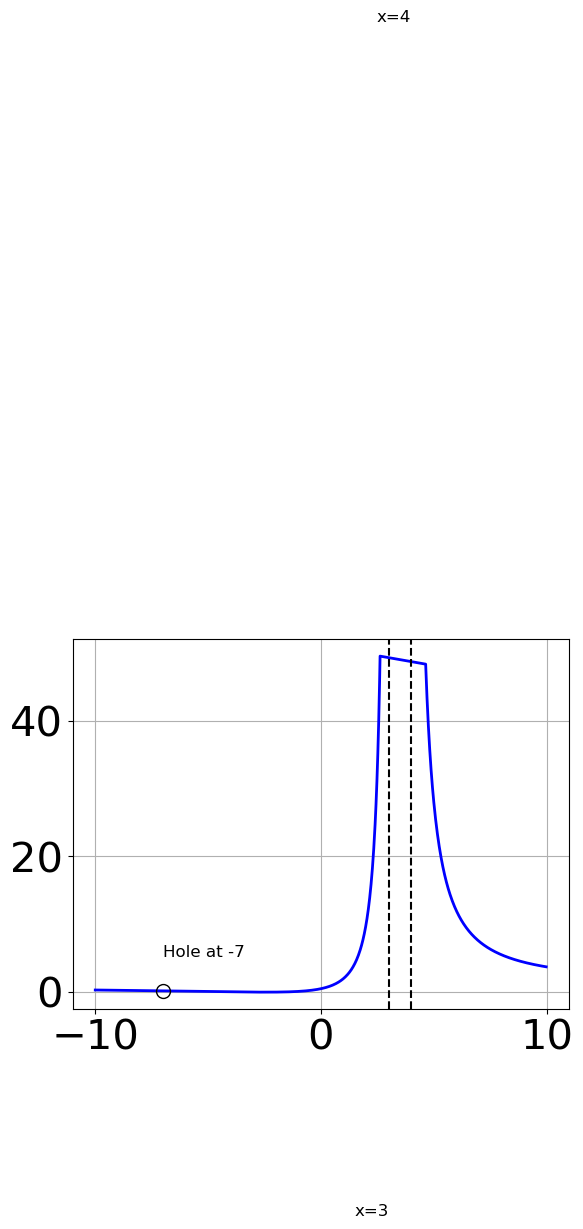
\includegraphics[width=0.5\textwidth]{../Figures/identifyGraphOfRationalFunctionCopyC.png}
\end{center}


The solution is \( f(x)=\frac{x^{3} +12.0 x^{2} +41.0 x + 42.0}{x^{3} -37.0 x + 84.0} \), which is option C.\begin{enumerate}[label=\Alph*.]
\item \( f(x)=\frac{x^{3} -11.0 x^{2} +36.0 x -36.0}{x^{3} -37.0 x -84.0} \)

You treated all of the zeros in the denominator as vertical asmptotes when some of them were holes and wrote factors as $x+z$.
\item \( f(x)=\frac{x^{3} -12.0 x^{2} +41.0 x -42.0}{x^{3} -37.0 x -84.0} \)

Remember that factors are written as $x-z$. For example, the zero $x=3$ corresponds to the factor $x-(3)$.
\item \( f(x)=\frac{x^{3} +12.0 x^{2} +41.0 x + 42.0}{x^{3} -37.0 x + 84.0} \)

This is the correct answer!
\item \( f(x)=\frac{x^{3} -19.0 x -30.0}{x^{3} -37.0 x + 84.0} \)

You treated all of the zeros in the denominator as vertical asymptotes when some of them were holes!
\item \( \text{None of the above are possible equations for the graph.} \)

If you believe none of the functions above could be the graph, please contact the coordinator.
\end{enumerate}

\textbf{General Comment:} We want to factor the numerator and denominator to determine which zeros in the denominator are vertical asympototes and which are holes.
}
\litem{
Determine the horizontal and/or oblique asymptotes in the rational function below.
\[ f(x) = \frac{9x^{3} +33 x^{2} -32 x -80}{3x^{2} +10 x -25} \]The solution is \( y = 3x + 1 \), which is option D.\begin{enumerate}[label=\Alph*.]
\item \( \text{Horizontal Asymptote at } y = -5.0 \)

This corresponds to considering where the denominator is equal to 0 as horizontal asymptote.
\item \( \text{Horizontal Asymptote of } y = 3.0 \text{ and Oblique Asymptote of } y = 3x + 1 \)

This corresponds to believing there can be both a horizontal and oblique asymptote.
\item \( \text{Horizontal Asymptote of } y = 3.0  \)

This corresponds to using rule for Horizontal Asymptote when degree of numerator and denominator match.
\item \( \text{Oblique Asymptote of } y = 3x + 1. \)

This is the correct answer.
\item \( \text{Horizontal Asymptote of } y = -5.0 \text{ and Oblique Asymptote of } y = 3x + 1 \)

This corresponds to believing there can be both a horizontal and oblique asymptote AND mixing up horizontal/vertical asymoptote.
\end{enumerate}

\textbf{General Comment:} We have a Horizontal Asymptote if the degree of the numerator is smaller than or equal to the degree of the denominator. We have an Oblique Asymptote if the degree of the numerator is larger than the degree of the denominator. We cannot have both!
}
\litem{
Which of the following functions \textit{could} be the graph below?

\begin{center}
    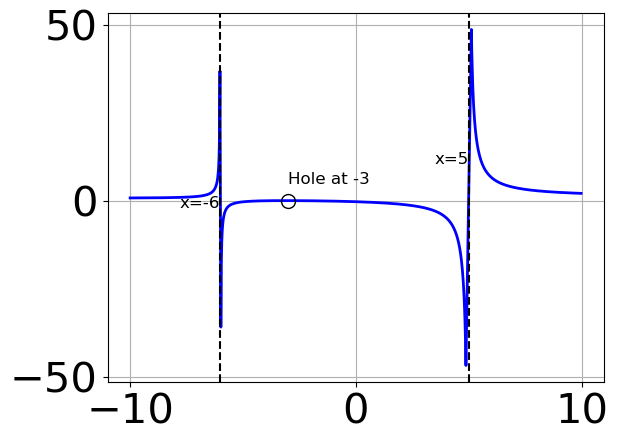
\includegraphics[width=0.5\textwidth]{../Figures/identifyGraphOfRationalFunctionC.png}
\end{center}


The solution is \( f(x)=\frac{x^{3} +9.0 x^{2} +26.0 x + 24.0}{x^{3} +4.0 x^{2} -27.0 x -90.0} \), which is option C.\begin{enumerate}[label=\Alph*.]
\item \( f(x)=\frac{x^{3} -9.0 x^{2} +26.0 x -24.0}{x^{3} -4.0 x^{2} -27.0 x + 90.0} \)

Remember that factors are written as $x-z$. For example, the zero $x=-6$ corresponds to the factor $x-(-6)$.
\item \( f(x)=\frac{x^{3} +5.0 x^{2} +2.0 x -8.0}{x^{3} +4.0 x^{2} -27.0 x -90.0} \)

You treated all of the zeros in the denominator as vertical asymptotes when some of them were holes!
\item \( f(x)=\frac{x^{3} +9.0 x^{2} +26.0 x + 24.0}{x^{3} +4.0 x^{2} -27.0 x -90.0} \)

This is the correct answer!
\item \( f(x)=\frac{x^{3} + x^{2} -34.0 x + 56.0}{x^{3} -4.0 x^{2} -27.0 x + 90.0} \)

You treated all of the zeros in the denominator as vertical asmptotes when some of them were holes and wrote factors as $x+z$.
\item \( \text{None of the above are possible equations for the graph.} \)

If you believe none of the functions above could be the graph, please contact the coordinator.
\end{enumerate}

\textbf{General Comment:} We want to factor the numerator and denominator to determine which zeros in the denominator are vertical asympototes and which are holes.
}
\litem{
Determine the vertical asymptotes and holes in the rational function below.
\[ f(x) = \frac{6x^{3} -23 x^{2} +29 x -12}{12x^{2} -7 x -12} \]The solution is \( \text{Vertical Asymptote of } x = -0.75 \text{ and hole at } x = 1.333 \), which is option E.\begin{enumerate}[label=\Alph*.]
\item \( \text{Vertical Asymptote of } x = 0.5 \text{ and hole at } x = 1.333 \)

This corresponds to mixing vertical and horizontal asymptotes.
\item \( \text{Vertical Asymptotes of } x = -0.75 \text{ and } x = 1.333 \text{ with no holes.} \)

This corresponds to not factoring out the hole.
\item \( \text{Holes at } x = -0.75 \text{ and } x = 1.333 \text{ with no vertical asymptotes.} \)

This corresponds to considering where the denominator is equal to 0 as holes.
\item \( \text{Vertical Asymptotes of } x = -0.75 \text{ and } x = 1.5 \text{ with a hole at } x = 1.333 \)

This corresponds to setting the numerator equal to 0.
\item \( \text{Vertical Asymptote of } x = -0.75 \text{ and hole at } x = 1.333 \)

This is the correct answer.
\end{enumerate}

\textbf{General Comment:} Remember to factor the numerator and denominator. Any factors that cancel are holes in the function. The zeros left in the denominator are the vertical asymptotes.
}
\litem{
Determine the horizontal and/or oblique asymptotes in the rational function below.
\[ f(x) = \frac{6x^{3} +5 x^{2} -49 x -60}{3x^{2} -5 x -12} \]The solution is \( y = 2x + 5 \), which is option A.\begin{enumerate}[label=\Alph*.]
\item \( \text{Oblique Asymptote of } y = 2x + 5. \)

This is the correct answer.
\item \( \text{Horizontal Asymptote at } y = 3.0 \)

This corresponds to considering where the denominator is equal to 0 as horizontal asymptote.
\item \( \text{Horizontal Asymptote of } y = 2.0 \text{ and Oblique Asymptote of } y = 2x + 5 \)

This corresponds to believing there can be both a horizontal and oblique asymptote.
\item \( \text{Horizontal Asymptote of } y = 2.0  \)

This corresponds to using rule for Horizontal Asymptote when degree of numerator and denominator match.
\item \( \text{Horizontal Asymptote of } y = 3.0 \text{ and Oblique Asymptote of } y = 2x + 5 \)

This corresponds to believing there can be both a horizontal and oblique asymptote AND mixing up horizontal/vertical asymoptote.
\end{enumerate}

\textbf{General Comment:} We have a Horizontal Asymptote if the degree of the numerator is smaller than or equal to the degree of the denominator. We have an Oblique Asymptote if the degree of the numerator is larger than the degree of the denominator. We cannot have both!
}
\litem{
Determine the horizontal and/or oblique asymptotes in the rational function below.
\[ f(x) = \frac{5x^{2} +7 x -6}{15x^{3} +16 x^{2} -5 x -6} \]The solution is \( \text{Horizontal Asymptote of } y = 0 \), which is option D.\begin{enumerate}[label=\Alph*.]
\item \( \text{Horizontal Asymptote at } y = -2.000 \)

This corresponds to considering where the denominator is equal to 0 as horizontal asymptote.
\item \( \text{Horizontal Asymptote of } y = 0.333  \)

This corresponds to using rule for Horizontal Asymptote when degree of numerator and denominator match.
\item \( \text{Horizontal Asymptote of } y = 0.333 \text{ and Oblique Asymptote of } y = 3x -1 \)

This corresponds to believing there can be both a horizontal and oblique asymptote.
\item \( \text{Horizontal Asymptote of } y = 0 \)

* This is the correct option.
\item \( \text{Oblique Asymptote of } y = 3x -1. \)

This corresponds to flipping the numerator and denominator, then using synthetic division to find the oblique asymptote.
\end{enumerate}

\textbf{General Comment:} We have a Horizontal Asymptote if the degree of the numerator is smaller than or equal to the degree of the denominator. We have an Oblique Asymptote if the degree of the numerator is larger than the degree of the denominator. We cannot have both!
}
\litem{
Determine the vertical asymptotes and holes in the rational function below.
\[ f(x) = \frac{6x^{3} +25 x^{2} +x -60}{6x^{2} +11 x -10} \]The solution is \( \text{Vertical Asymptote of } x = 0.667 \text{ and hole at } x = -2.5 \), which is option E.\begin{enumerate}[label=\Alph*.]
\item \( \text{Vertical Asymptotes of } x = 0.667 \text{ and } x = -2.5 \text{ with no holes.} \)

This corresponds to not factoring out the hole.
\item \( \text{Vertical Asymptote of } x = 1.0 \text{ and hole at } x = -2.5 \)

This corresponds to mixing vertical and horizontal asymptotes.
\item \( \text{Holes at } x = 0.667 \text{ and } x = -2.5 \text{ with no vertical asymptotes.} \)

This corresponds to considering where the denominator is equal to 0 as holes.
\item \( \text{Vertical Asymptotes of } x = 0.667 \text{ and } x = 1.333 \text{ with a hole at } x = -2.5 \)

This corresponds to setting the numerator equal to 0.
\item \( \text{Vertical Asymptote of } x = 0.667 \text{ and hole at } x = -2.5 \)

This is the correct answer.
\end{enumerate}

\textbf{General Comment:} Remember to factor the numerator and denominator. Any factors that cancel are holes in the function. The zeros left in the denominator are the vertical asymptotes.
}
\litem{
Determine the vertical asymptotes and holes in the rational function below.
\[ f(x) = \frac{8x^{3} -22 x^{2} +3 x + 18}{6x^{2} +x -15} \]The solution is \( \text{Vertical Asymptote of } x = -1.667 \text{ and hole at } x = 1.5 \), which is option C.\begin{enumerate}[label=\Alph*.]
\item \( \text{Vertical Asymptotes of } x = -1.667 \text{ and } x = -0.75 \text{ with a hole at } x = 1.5 \)

This corresponds to setting the numerator equal to 0.
\item \( \text{Vertical Asymptotes of } x = -1.667 \text{ and } x = 1.5 \text{ with no holes.} \)

This corresponds to not factoring out the hole.
\item \( \text{Vertical Asymptote of } x = -1.667 \text{ and hole at } x = 1.5 \)

This is the correct answer.
\item \( \text{Holes at } x = -1.667 \text{ and } x = 1.5 \text{ with no vertical asymptotes.} \)

This corresponds to considering where the denominator is equal to 0 as holes.
\item \( \text{Vertical Asymptote of } x = 1.333 \text{ and hole at } x = 1.5 \)

This corresponds to mixing vertical and horizontal asymptotes.
\end{enumerate}

\textbf{General Comment:} Remember to factor the numerator and denominator. Any factors that cancel are holes in the function. The zeros left in the denominator are the vertical asymptotes.
}
\end{enumerate}

\end{document}